%\part{Montagem de Hardware}


\chapter[DESIGN DO SISTEMA]{Design do Sistema}

A rede de transmissão de dados terá a arquitetura apresentada na figura [\ref{Fig: rede ponto a ponto}], sendo capaz de transmitir dados unidirecionalmente de um ponto a outro. O canal de comunicação é o meio aéreo.

\begin{figure}
	\centering
		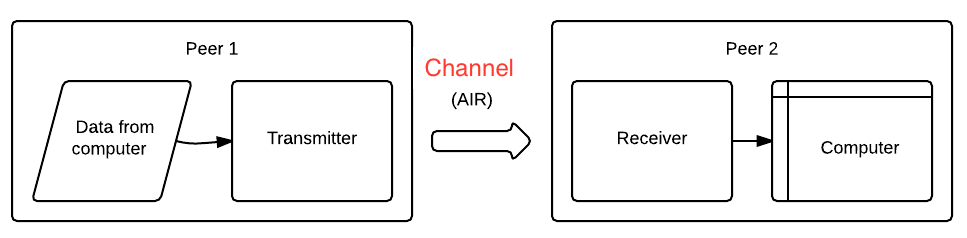
\includegraphics[keepaspectratio=true scale=0.3]{figuras/network-connection}
	\caption{Configuração da rede de comunicação ponto a ponto.}
	\label{Fig: rede ponto a ponto}
\end{figure}

O diagrama de blocos mais detalhado do mecanismo de transmissão é apresentado na figura [\ref{Fig: Esquema simplificado da transmissão de dados}]. O primeiro bloco representa a mensagem a ser transmitida. De posse da mensagem , temos que codificá-la de modo que a possa ser transmitida pelo canal de comunicação aéreo. Temos diversas maneiras de adquirir e armazenar a mensagem, e a mesma pode se encontrar em diversos formatos como binário, áudio, vídeo dentre outros.

\begin{figure}
	\centering
		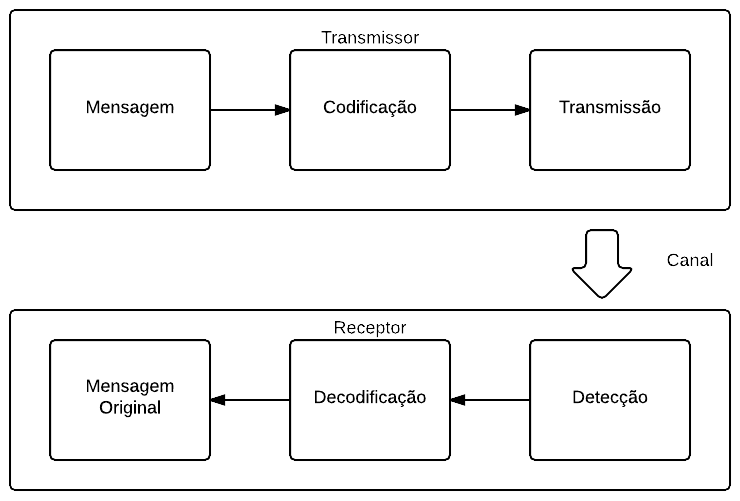
\includegraphics[keepaspectratio=true scale=0.3]{figuras/diagrama_transmissao}
	\caption{Esquema simplificado da transmissão de dados.}
	\label{Fig: Esquema simplificado da transmissão de dados}
\end{figure}

Atualmente possuímos múltiplos meios de entrada em um sistema, porém iremos reduzir os nossos testes a três métodos de entrada, começando por informações pré-programadas dentro do microcontrolador, passando por entradas de usuário via teclado e finalmente será testado o envio de aquivos entre os dois pontos de comunicação.
 
O transmissor estará exposto ao ambiente interno, uma sala por exemplo. O ar será o canal de transmissão por onde a luz deverá viajar. 

O receptor é composto pelo elemento de detecção de luz, que transformará os fótons em sinais elétricos. Estes sinais, por vez, devem ser decodificados em código binário que possibilita a reconstrução da mensagem original.

\section{Codificaçao do Canal}

O canal de comunicação, ar, no entanto é o responsável pela introdução de ruído, interferências e por corromper a mensagem. E esses erros podem ser devido a diferentes fatores como por exemplo obstáculos, luz externa e outras fontes de interferência. Desta maneira podem ocorrer uma série de discrepâncias nos bits recebidos com relação aos bits enviados.
Uma das maneiras de garantir a integridade do sinal transmitido é o uso de técnicas de codificação de canal. O principal objetivo dessa técnica é reduzir o SNR (\textit{Signal to Noise Ratio}), aumentado a eficiência do canal de transmissão.
A grande vantagem da codificação de canal é portanto melhorar o desempenho do sistema em relação a uma transmissão não codificada.
As técnicas de codificação de canal consistem genericamente na introdução de bits redundantes na informação a transmitir. Os bits adicionais permitem, de um modo geral, a detecção e em alguns casos a correção de erros nos bits recebidos. O meio mais simples de se detectar erros na transmissão de uma mensagem e a adição de um bit de paridade. 
Existem dois tipos de códigos de paridade, o par e o impar. Na paridade par, é adicionado um bit \lq 1\rq \: ou \lq 0\rq \: ao inicio ou ao final da mensagem de forma a obter um numero par de bits \lq 1s\rq \: na mesma, já na paridade ímpar, o bit é adicionado para se obter um numero ímpar de bits \lq 1s\rq.

Contudo o uso das técnicas de codificação tem um preço, quando reduzimos o tamanho da informação útil para adicionar redundâncias estamos reduzindo a largura de banda da nossa comunicação em prol de um sistema mais seguro. 

\section{Codificação de Linha}

A codificação de linha consiste em representar sinais digitais por formas de onda banda base. Uma maneira simples de codificar bits em pulsos é o chaveamento \textit{On-Off} (OOK), que representa o bit \lq 1\rq \: pela presença de um nível DC e o bit \lq 0\rq \: pela ausência dele, como mostrado na figura [\ref{Fig: ook}].

\begin{figure}
	\centering
		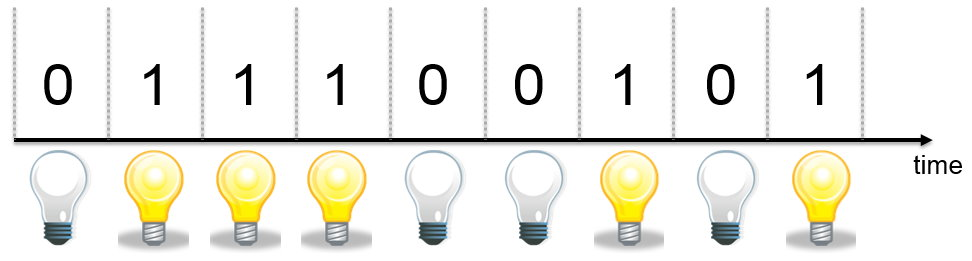
\includegraphics[width = 12cm]{figuras/ook}
	\caption{Codificação \textit{On-Off Keying}.}
	\label{Fig: ook}
\end{figure}

Por fim a mensagem enviada terá o formato do pacote figura[\ref{Fig: pacote}].

\begin{figure}
	\centering
		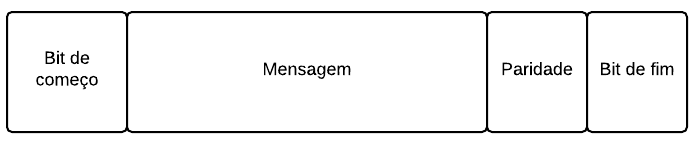
\includegraphics[width = 12cm]{figuras/pacote}
	\caption{Pacote de dados enviados.}
	\label{Fig: pacote}
\end{figure}

\section{Transmissor Óptico}

O transmissor óptico converte o sinal elétrico em luz, e projeta este sinal no canal de transmissão. Este sistema consiste em uma fonte de fótons, e sistemas auxiliares para operar a fonte de luz.
O primeiro passo no design do \textit{hardware} de transmissão é decidir qual será a fonte de fótons a ser utilizada, pois todo \textit{hardware} tem que ser projetado para que o possa ser suportada a fonte de luz escolhida.

A segunda parte do transmissor é composta por um \textit{software} que é o responsável por captar os dados, converter para binário e encapsular toda a informação necessário ao pacote. 
A mensagem útil (\textit{payload}) é encapsulada por vários bits. Estes bits sobressalentes a mensagem indicam o início do \textit{stream}, o final e a codificação de linha que irá indicar erros nos pacotes recebidos figura [\ref{Fig: pacote}].

Para que o \textit{hardware} e \textit{software} funcionem bem é imprescindível que as limitações de cada sistema seja conhecida, para que haja otimização das taxas de transferência de dados e redução dos erros (BER).
 
\subsection{Emissor de fóton}

A escolha do emissor de fótons influência em todo o projeto do transmissor, e a correta seleção do elemento emissor de luz é imprescindível para o sucesso do transmissão de dados. 
Existem duas tecnologias básicas sendo utilizadas na comunicação óptica hoje em dia, uma vertente faz o uso dos LEDs, e a outra de lasers (LDs).
É importante ressaltar que os lasers não podem ser utilizados para a finalidade de iluminação devido ao risco aos olhos. Fora detalhes que impedem que esta tecnologia seja utilizada na iluminação de ambientes como o fato de sua luz ser monocromática e seu feixe de luz ser estreito, não se qualificando para uso em VLCs.

\subsubsection{Diodos Emissores de Luz (LEDs)}

Os diodos emissores de luz ou mais popularmente LEDs são fontes ópticas formados por uma
junção p-n. O semicondutor \textit{p} tem falta de cargas negativas, que podem ser chamados de lacunas e o semicondutor \textit{n} excesso de cargas negativas na forma de elétrons figura[\ref{Fig: juncao-pn}]. \cite{Razavi}

\begin{figure}
	\centering
		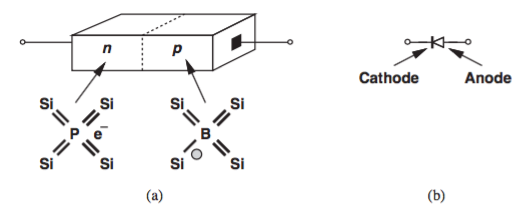
\includegraphics[width = 12cm]{figuras/juncao-pn}
	\caption{Junção p-n de um diodo.\cite{Razavi}}
	\label{Fig: juncao-pn}
\end{figure}


Ao aplicar tensão direta na junção p-n, os elétrons entram num estado de excitação que é instável. Quando os elétrons energizados retornam ao estado estável, eles liberam energia na forma de fóton. 
Os fótons podem ser da faixa infravermelha, visível ou ultravioleta de acordo com o material semicondutor utilizado. Essa característica de comprimento de onda está relacionado com o \textit{gap} de energia do material semicondutor. A energia do fóton emitido é aproximadamente igual a diferença entre a banda de condução e a banda de valência, isto é, o \textit{gap} de energia.

Adicionalmente, desde que os fótons são somente liberados quando os elétrons se combinam com lacunas, se mais elétrons e lacunas se recombinarem, mais fótons serão emitidos. Isso significa que a emissão de luz dos LEDs pode ser aproximada linearmente com relação a corrente que é aplicada entre seus terminais.

LEDs possuem algumas características importantes como o comprimento de onda do fótons emitidos, ou seja a cor da luz emitida, é determinada pela banda de valência do semicondutor. A largura do espectro de saída pode variar até 50 $\eta$m ao redor do comprimento de onda central, que é ditado pela banda de valência.

A velocidade de chaveamento de um LED é determinado pela constante de tempo de recombinação. Dependendo do \textit{design}, o tempo de subida, \textit{rise time}, pode variar entre 1 e 100 $\eta$s \cite{friedman}, o que significa que os LEDs podem alcançar frequências de chaveamento de até centenas de MHz.


\subsection{Escolha do Dispositivo Óptico}

A decisão feita levou em consideração o foco principal do projeto, que é poder conciliar a transmissão de dados a sistemas de iluminação existentes, sejam de carros, casas ou outros ambientes. O que pode ser atingido com o uso dos dispositivos baseados na tecnologia LED. Visto que o dispersão de luz assim como o comprimento de onda são mais abertos em relação ao laser.
Outras características também contaram para a escolha deste dispositivo como: 

\begin{itemize}
\item Podem ser modulados em altas velocidades.
\item Baixo custo.
\item Circuito \textit{driver} de baixa complexidade.
\item Fácil aquisição no mercado.
\item Seguro aos olhos humanos.
\item Luz não coerente.
\item Amplo ângulo de transmissão.
\end{itemize}

\subsection{\textit{Driver} do LED}

Uma vez escolhido o dispositivo fonte de luz, o próximo passo é determinar como será feita a modulação do sinal, ligar e desligar o LED, em relação a informação binária. Como os LEDs são dispositivos controlados por corrente o seu controle será feito por uma fonte de corrente contínua com resistor em série para limitar a amperagem. 
A título de teste e prova de conceito do sistema de comunicação VLC, o circuito foi montado figura [\ref{Fig: sistema-transmissao}] para alimentar o diodo. Como o LED utilizado é de baixa potência, a corrente e tensão fornecidas pelo microcontrolador são suficientes para o correto funcionamento do emissor de luz.

\begin{figure}
	\centering
		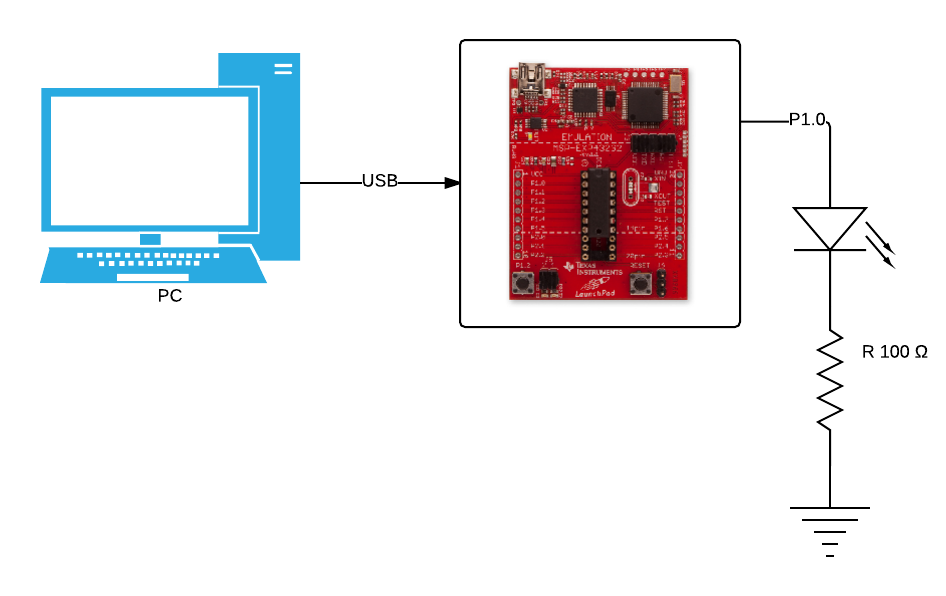
\includegraphics[width = 12cm]{figuras/sistema-transmissao}
	\caption{Sistema de transmissão com microcontrolador alimentando o LED de baixa potência.}
	\label{Fig: sistema-transmissao}
\end{figure}

\subsection{Mensagem}

Agora o sistema carece de uma fonte de sinal para ser convertido em binário e 
consequentemente enviada ao driver responsável por estimular o LED.
Para efeito de teste foram utilizados dois métodos de entrada para o sistema descrito na 
figura [\ref{Fig: sistema-transmissao}], o primeiro se utiliza de uma mensagem 
pré compilada no microcontrolador, sem a necessidade de outros periféricos. Esta abordagem 
é muito útil para fins de teste, pois o usuário não pode intervir em nenhuma parte do 
processo, isolando fontes de erros.
A segunda fase de testes contou com a aquisição de dados via computador, os quais podem 
ser tanto via a entrada padrão de teclado e até mesmo arquivos de qualquer tipo, como fotos, arquivos de texto, áudio ou vídeo. 

O arquivo então é transferido serialmente via USB do computador para o controlador utilizando o protocolo UART. O microprocessador é o dispositivo responsável por codificar e inserir os bits restantes de informação ao pacote de dados, como mostrado na figura [\ref{Fig: pacote}]. Para o teste foram utilizados dois controladores diferentes o Texas MSP430 e o Arduino ATmega 328, ambos com clock de 16 MHz.


\subsection{Teste do emissor}

A figura[\ref{Fig: sistema-transmissao}] mostra o sistema de transmissão. A informação é
enviada pelo computador para o controlador via cabo USB, utilizando o protocolo de 
comunicação UART. O controlador recebe um bloco de informações via serial e os armazena em um buffer interno. O pacote a ser transmitido é convertido em binário e enviado ao circuito responsável por acionar o LED.


\subsection{Futuros aprimoramentos do emissor}

O diodo emissor de luz utilizado nos testes possui baixa potência o que nos leva a escolher um
novo LED capaz de realizar uma melhor iluminação do ambiente. Para chavear um LED de maior 
potencia é necessário o \textit{design} de um novo circuito de alimentação capaz de comutar 
rapidamente e fornecer níveis de corrente apropriados. 

Tendo em vista a melhora da transmissão, e possibilidade de utilizar modulações avançadas a inclusão de um conversor DAC é indispensável, resultando em um novo diagrama de transmissão apresentado na figura [\ref{Fig: sistema-futuro-transmissao}].

 \begin{figure}
	\centering
		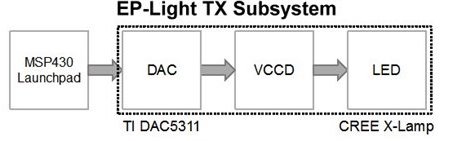
\includegraphics[width = 12cm]{figuras/sistema-futuro-transmissao}
	\caption{Sistema de transmissão com conversor digital analógico e circuito chaveador de LED de alta potência.}
	\label{Fig: sistema-futuro-transmissao}
\end{figure}

O sinal convertido pelo DAC estimulará o driver VCCD, que é uma fonte de corrente controlado por tensão, responsável por ligar e desligar o diodo LED.

\section{Receptor Óptico}

O sistema de recepção detecta o sinal óptico e o transforma em um sinal elétrico. Este sistema consiste de um detector de fótons, o qual converte um sinal óptico em corrente elétrica, e hardware capaz de transformar os sinais elétricos captados em informação útil e que possa ser compreendida pelo usuário do sistema.

Assim como no transmissor, o componente óptico determina todo o sistema de recepção, neste caso o detector de fótons. Para a finalidade de transmissão de dados este componente óptico deve atender a alguns requisitos a serem explicados na próxima subseção.

\subsection{Detector de fóton}

Existem muitos tipos diferentes de dispositivos opto-eletrônicos que podem ser utilizados como fotodetectores. Idealmente um fotodetector deve ser capaz de responder rapidamente a estímulos de fótons realizada pelo transmissor sem que seja adicionado ruido ao sinal. Adicionalmente este dispositivo deve ser pequeno, robusto e barato. Infelizmente o dispositivo real não cumprirá todos estes aspectos, para a nossa aplicação a velocidade de chaveamento é o quesito de maior importância para a escolha do detector, seguido pela sensibilidade a luz emitida. 

\subsubsection{p-n Fotodiodo}

Fotodiodos convertem luz em corrente elétrica. A incidência de luz, em um semicondutor produz agitação térmica que liberam pares de elétrons e buracos em vários pontos no diodo, como ilustrado na figura [\ref{Fig: fotodiodo}]. Esses postadores se direcionam rumo a extremos opostos do dispositivo sob a influência do campo aplicado. Em resumos quando a luz incide no fotodiodo, uma corrente é gerada do cátodo para o ânodo. \cite{Razavi}

 \begin{figure}
	\centering
		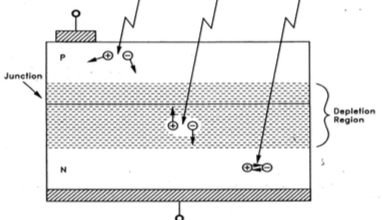
\includegraphics[width = 12cm]{figuras/fotodiodo}
	\caption{Luz provoca agitação das cargas livres no fotodiodo que geram a recombinação de pares elétrons lacuna.}
	\label{Fig: fotodiodo}
\end{figure}

Estes dispositivos, assim como os diodos, consistem de duas camadas de semicondutores uma do tipo \lq n\rq \: e outra \lq p\rq \:. Fotodiodos apresentam na camada do tipo \lq p\rq \: excesso de lacunas e na camada do tipo \lq n\rq \: excesso de elétrons figura [\ref{Fig: juncao-pn}]. Na região de junção dos dois substratos é criada uma região de depleção. Nesta região elétrons e lacunas se recombinam para equalizar o número de portadores livres no semicondutor. Este fenômeno produz carga positiva no material tipo \lq n\rq \: e carga negativa no material do tipo \lq p\rq \: , devido a redução do número de elétrons e lacunas livres. 
A existência dessa carga previne que mais buracos atravessem a zona de depleção em direção a zona de elétrons livres no material tipo \lq n\rq \: . \cite{alexanderstephenb.1997}


Quando a luz passa através um diodo, esse fóton pode excitar um elétron, criando um par de elétron e uma lacuna. Se isto ocorrer perto da zona de depleção, o campo elétrico irá guiar lacunas em direção ao ânodo, lado \lq p\rq \:, e elétrons em direção ao lado \lq n\rq \: . Essa separação de cargas leva a uma diferença de potencial entre as junções pn. Esse potencial produz a chamada fotocorrente.\cite{scherzpaul2007}

O campo elétrico resultante da zona de depleção é aumentado se aplicado campo elétrico na polarização reversa do diodo. E um campo elétrico maior produz uma zona de depleção maior, o que 
aumenta significativamente a eficiência quântica, o que significa que o dispositivo será mais sensível a 
luz de acordo com a equação [\ref{Eq: eficiencia_fotodiodo}]. Uma região de depleção maior implica em redução da capacitância da junção, porém também aumenta o tempo que pares de elétrons e lacunas levam para atravessar a zona de depleção, reduzindo a largura de banda. \cite{alexanderstephenb1997}

\begin{equation}
\label{Eq: eficiencia_fotodiodo}
\eta = \frac{número\: de\: portadores\: prduzidos}{número\: de \:fótons\: incidentes}
\end{equation}

Como cada fóton somente pode excitar no máximo um elétron, e os fotodiodos não possuem nenhum tipo de ganho interno, isso conta como um ponto negativo. Em troca tais dispositivos possuem incrível linearidade, e tempo de subida (\textit{rise time}) de até 10 $\rho$s, são relativamente
imunes a ruido e possuem baixo custo. \cite{eg&goptoelectronics1997}

\begin{table}[h]
	\centering
	\begin{tabular}{cc}
		\toprule
		\textbf{Propriedades fotodiodo} & \textbf{Valores} \\
		\midrule
		$\lambda$ máx. sensibilidade & 850 nm\\
		Sensibilidade & 400 - 1100 nm \\
		Meio ângulo $\varphi$ & $\pm$ $10^{\circ}$  \\
		Tempo de subida e descida & 0,005 $\mu$s\\
		\bottomrule
	\end{tabular}
	\caption{Características do fotodiodo utilizado. \cite{osramoptosemiconductors2014}}
	\label{Tab: caracteristicas fotodiodo}
\end{table}

O fotodiodo apresentado na tabela [\ref{Tab: caracteristicas fotodiodo}] se encaixa perfeitamente nos quesitos exigidos por um receptor. Tem sensibilidade que cobre a faixa de espectro visivel pelo ser humano 400 - 700 $\eta$m, baixo tempo de subida, porém estreito ângulo de detecçao. O tempo de subida apresentado viabiliza uma taxa de comunicaçao teórica na faixa das centenas de Mbps.

\subsection{Processamento do sinal}

O objetivo do receptor óptico é recuperar a mensagem original que foi enviada, e para isso temos que percorrer o caminho inverso do sistema de transmissão.
Sabendo como o componente de detecção de luz funciona, podemos projetar o \textit{hardware} eletrônico responsável por condicionar o sinal recebido pelo detector óptico. 
A figura [\ref{Fig: recepcao}] mostra os principais blocos utilizados no receptor.

 \begin{figure}
	\centering
		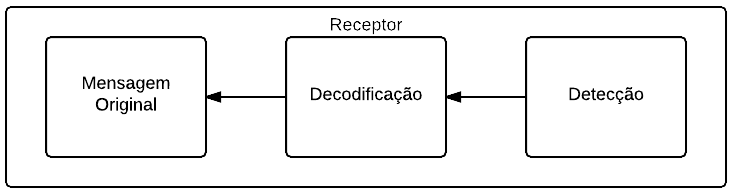
\includegraphics[width = 12cm]{figuras/diagrama_recepcao}
	\caption{Processo de reconstrução da mensagem original.}
	\label{Fig: recepcao}
\end{figure}

O primeiro passo é detectar o sinal com o fotodiodo. Este dispositivo excita corrente entre os seus terminais, porém os controladores não são capazes de ler níveis de corrente, então por este motivo teremos um conversor corrente-tensão que irá converter a amperagem em níveis de tensão que podem ser lidos pelo processador. Por fim os sinais sem muito significado inicialmente podem ser decodificados, o processo de decodificação consiste em extrair o bit de começo e final da mensagem e comparar a paridade do pacote em busca de erros. Se for verificado que não possuem erros na mensagem recebida a mensagem reconstruída deve apresentar o mesmo conteúdo do pacote enviado.

\subsubsection{Conversor de Corrente - Tensão}

Como discutido anteriormente os fotodiodos funcionam como fonte de corrente quando expostos a luz. Apesar do sinal de corrente ser praticamente linear, a maioria dos componentes eletrônicos trabalham baseados em diferença de tensão. Por este motivo, o sinal de corrente proveniente do diodo deve primeiramente ser convertido em voltagem. 

Para o propósito de validação de conceito será montado um \textit{hardware} sem muita complexidade, porém completamente funcional e que seja capaz de simular a comunicação utilizando a tecnologia emergente VLC.

\begin{figure}
	\centering
		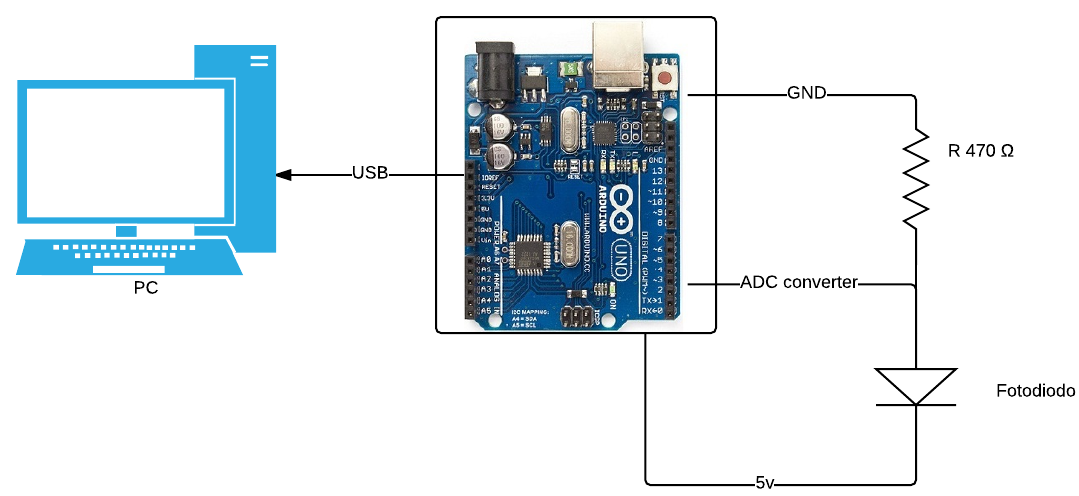
\includegraphics[keepaspectratio=true scale=0.3]{figuras/sistema_recepcao}
	\caption{Sistema de aquisição de dados ópticos.}
	\label{Fig: Aquisição de dados ópticos}
\end{figure}


O circuito da figura[\ref{Fig: Aquisição de dados ópticos}] foi utilizado nos testes. Quando a luz incide no diodo, uma corrente passa pelo resistor, e seguindo a lei de Ohm equação [\ref{Eq: lei de ohm}], esta corrente que atravessa o resistor será inversamente proporcional a tensão ente os seus terminais.

\begin{equation}
Voltagem\:[V] = \frac{Resistência\: [\Omega]}{Corrente\: [A]}
\label{Eq: lei de ohm}
\end{equation}

Temos então um circuito capaz de transformar corrente em sinais de tensão.

\subsubsection{Decodificação}

A etapa final é a conversão do sinal de tensão em informação útil ao usuário do sistema. Para realizar tal tarefa foi utilizado o um conversor analógico digital de 10 bits para, presente no microcontrolador ATmeaga 328. Este ADC converte os níveis de tensão de entrada, de 0 a 5 volts, em 1024 faixas.

O sinal de entrada pode possuir 1023 diferentes níveis lógicos, porém a informação que queremos somente dois níveis, chamada informação binária. 
Com o objetivo de converter a entrada analógica de vário níveis em binário devemos estabelecer um nível de \textit{threshold}. O \textit{threshold} funcionará como um parâmetro que determina se a informação de entrada é um bit \lq 1\rq \: ou um bit \lq 0\rq \:. Para valores abaixo do nível selecionado a informação será interpretada com um \lq zero\rq \: e níveis acima do selecionado são interpretados como o bit \lq um\rq \:.

Ao utilizar um limiar para definir se o bit de entrada é um nível alto, ou um nível baixo conferimos maior robustez às falhas visto que mesmo com a variações mínimas da luminosidade do sinal de entrada o bit ainda será reconhecido como zero ou um.

A pacote binário pode então ser processado pelo controlador e enviar ao computador via cabo USB.

\subsection{Futuros aprimoramentos do receptor}

São necessárias diversas melhorias no sistema de recepção de sinal óptico. O primeiro é a implementação de um sensor óptico com ângulo de detecção mais aberto o que não requer a o perfeito alinhamento do receptor e transmissor.
Da mesma maneira que foi utilizado um artifício elétrico para realizar a leitura da corrente gerada pelo fotodiodo, tem se como objetivo implementar um TIA (\textit{Transimpedance Amplifier}) que converte corrente em tensão, seguido pelo condicionamento da tensão do sinal de entrada e binarização da mensagem, como apresentado na figura[\ref{Fig: Receptor futuro}].

\begin{figure}
	\centering
		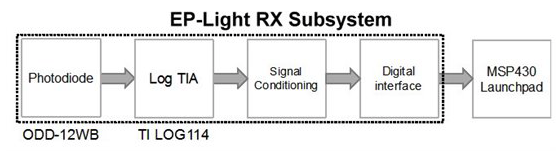
\includegraphics[width=12cm]{figuras/sistema-futuro-recepcao}
	\caption{Receptor futuro.}
	\label{Fig: Receptor futuro}
\end{figure}


Futuras melhorias serão realizadas a nível de hardware e software para conferir maior robustes ao sistema Rx e Tx.
